% moving it to vscode for copilot refining

\section{Data source and data description}

In this section, we demonstrate the functionality of \texttt{iClusterVB} for integrative clustering and feature selection using a simulated multi-omic dataset. This simulation is designed to closely mimic the structure of real-world biological data typically encountered in genomics and precision medicine studies.

The simulated dataset includes data from \( N = 240 \) individuals, each with measurements across \( R = 4 \) different data types. Specifically, two of these data types represent \textbf{continuous variables}---such as gene or mRNA expression levels---while the third data type consists of \textbf{count data}, resembling DNA copy number variations. The fourth data type is \textbf{binary}, capturing the presence or absence of mutations or other genomic aberrations. This combination of data types reflects a common setup in integrative genomic analyses, where multiple omic layers are collected for each subject.

We assume that the underlying true structure of the data consists of \( K = 4 \) distinct clusters, corresponding to four biological subgroups. These clusters are \textbf{balanced in size}, meaning each cluster contains 25\% of the individuals (\( \pi_1 = \pi_2 = \pi_3 = \pi_4 = 0.25 \)).

Each data type contains \( p_r = 500 \) features, for a total of \( p = 2000 \) features across all data types. Among these, \textbf{only 10\%} (i.e., 50 features per data type) are informative and contribute to the clustering structure. These informative features are also referred to as \textbf{relevant or discriminative features}, as they capture the variations that distinguish between clusters. The remaining 90\% of the features in each data type serve as \textbf{irrelevant noise features}, which do not contribute to the clustering and are expected to be filtered out during the feature selection process.

The distribution of these useful features across the four clusters is structured, and the table below summarizes how the relevant features are assigned within each cluster and data type.

\begin{table}[ht]
\centering
\caption{Distribution of relevant and noise features across clusters in each data view of the simulated data}
\label{tab:simulated_data}
\begin{tabular}{|l|l|l|}
\hline
\textbf{Data View} & \textbf{Cluster} & \textbf{Distribution} \\
\hline
\multirow{5}{*}{1 (Continuous)} 
& Cluster 1 & $\mathcal{N}(10, 1)$ (Relevant) \\
& Cluster 2 & $\mathcal{N}(5, 1)$ (Relevant) \\
& Cluster 3 & $\mathcal{N}(-5, 1)$ (Relevant) \\
& Cluster 4 & $\mathcal{N}(-10, 1)$ (Relevant) \\
& -         & $\mathcal{N}(0, 1)$ (Noise) \\
\hline
\multirow{5}{*}{2 (Continuous)} 
& Cluster 1 & $\mathcal{N}(-10, 1)$ (Relevant) \\
& Cluster 2 & $\mathcal{N}(-5, 1)$ (Relevant) \\
& Cluster 3 & $\mathcal{N}(5, 1)$ (Relevant) \\
& Cluster 4 & $\mathcal{N}(10, 1)$ (Relevant) \\
& -         & $\mathcal{N}(0, 1)$ (Noise) \\
\hline
\multirow{5}{*}{3 (Binary)} 
& Cluster 1 & Bernoulli(0.05) (Relevant) \\
& Cluster 2 & Bernoulli(0.2) (Relevant) \\
& Cluster 3 & Bernoulli(0.4) (Relevant) \\
& Cluster 4 & Bernoulli(0.6) (Relevant) \\
& -         & Bernoulli(0.1) (Noise) \\
\hline
\multirow{5}{*}{4 (Count)} 
& Cluster 1 & Poisson(50) (Relevant) \\
& Cluster 2 & Poisson(35) (Relevant) \\
& Cluster 3 & Poisson(20) (Relevant) \\
& Cluster 4 & Poisson(10) (Relevant) \\
& -         & Poisson(2) (Noise) \\
\hline
\end{tabular}
\end{table}

\subsection{Exploratory Data Analysis (EDA)}

To identify and visualize the valid normal distributions from the simulated dataset, we performed the following sampling and testing operations:

\begin{itemize}
    \item \textbf{Random Sampling:} We randomly sampled 30 variables from each of the three different distributions (normal, poisson, and multinomial), resulting in a total of 90 variables for testing.
    \item \textbf{Statistical Testing:} For each sampled variable, we conducted the corresponding statistical tests:
    \begin{itemize}
        \item A normality test (e.g., Shapiro-Wilk test) for variables assumed to follow a normal distribution.
        \item A Poisson test for variables assumed to follow a Poisson distribution.
        \item A multinomial test for variables assumed to follow a multinomial distribution.
    \end{itemize}
    \item \textbf{Validation and Visualization:} Variables that passed their respective tests were visualized to determine whether they represent truly valid features or are merely low-probability events arising from noise distributions.
\end{itemize}

This process helps to filter out irrelevant noise features and retain only the informative variables that contribute to the clustering structure.


\begin{figure}[!h]
    \centering
    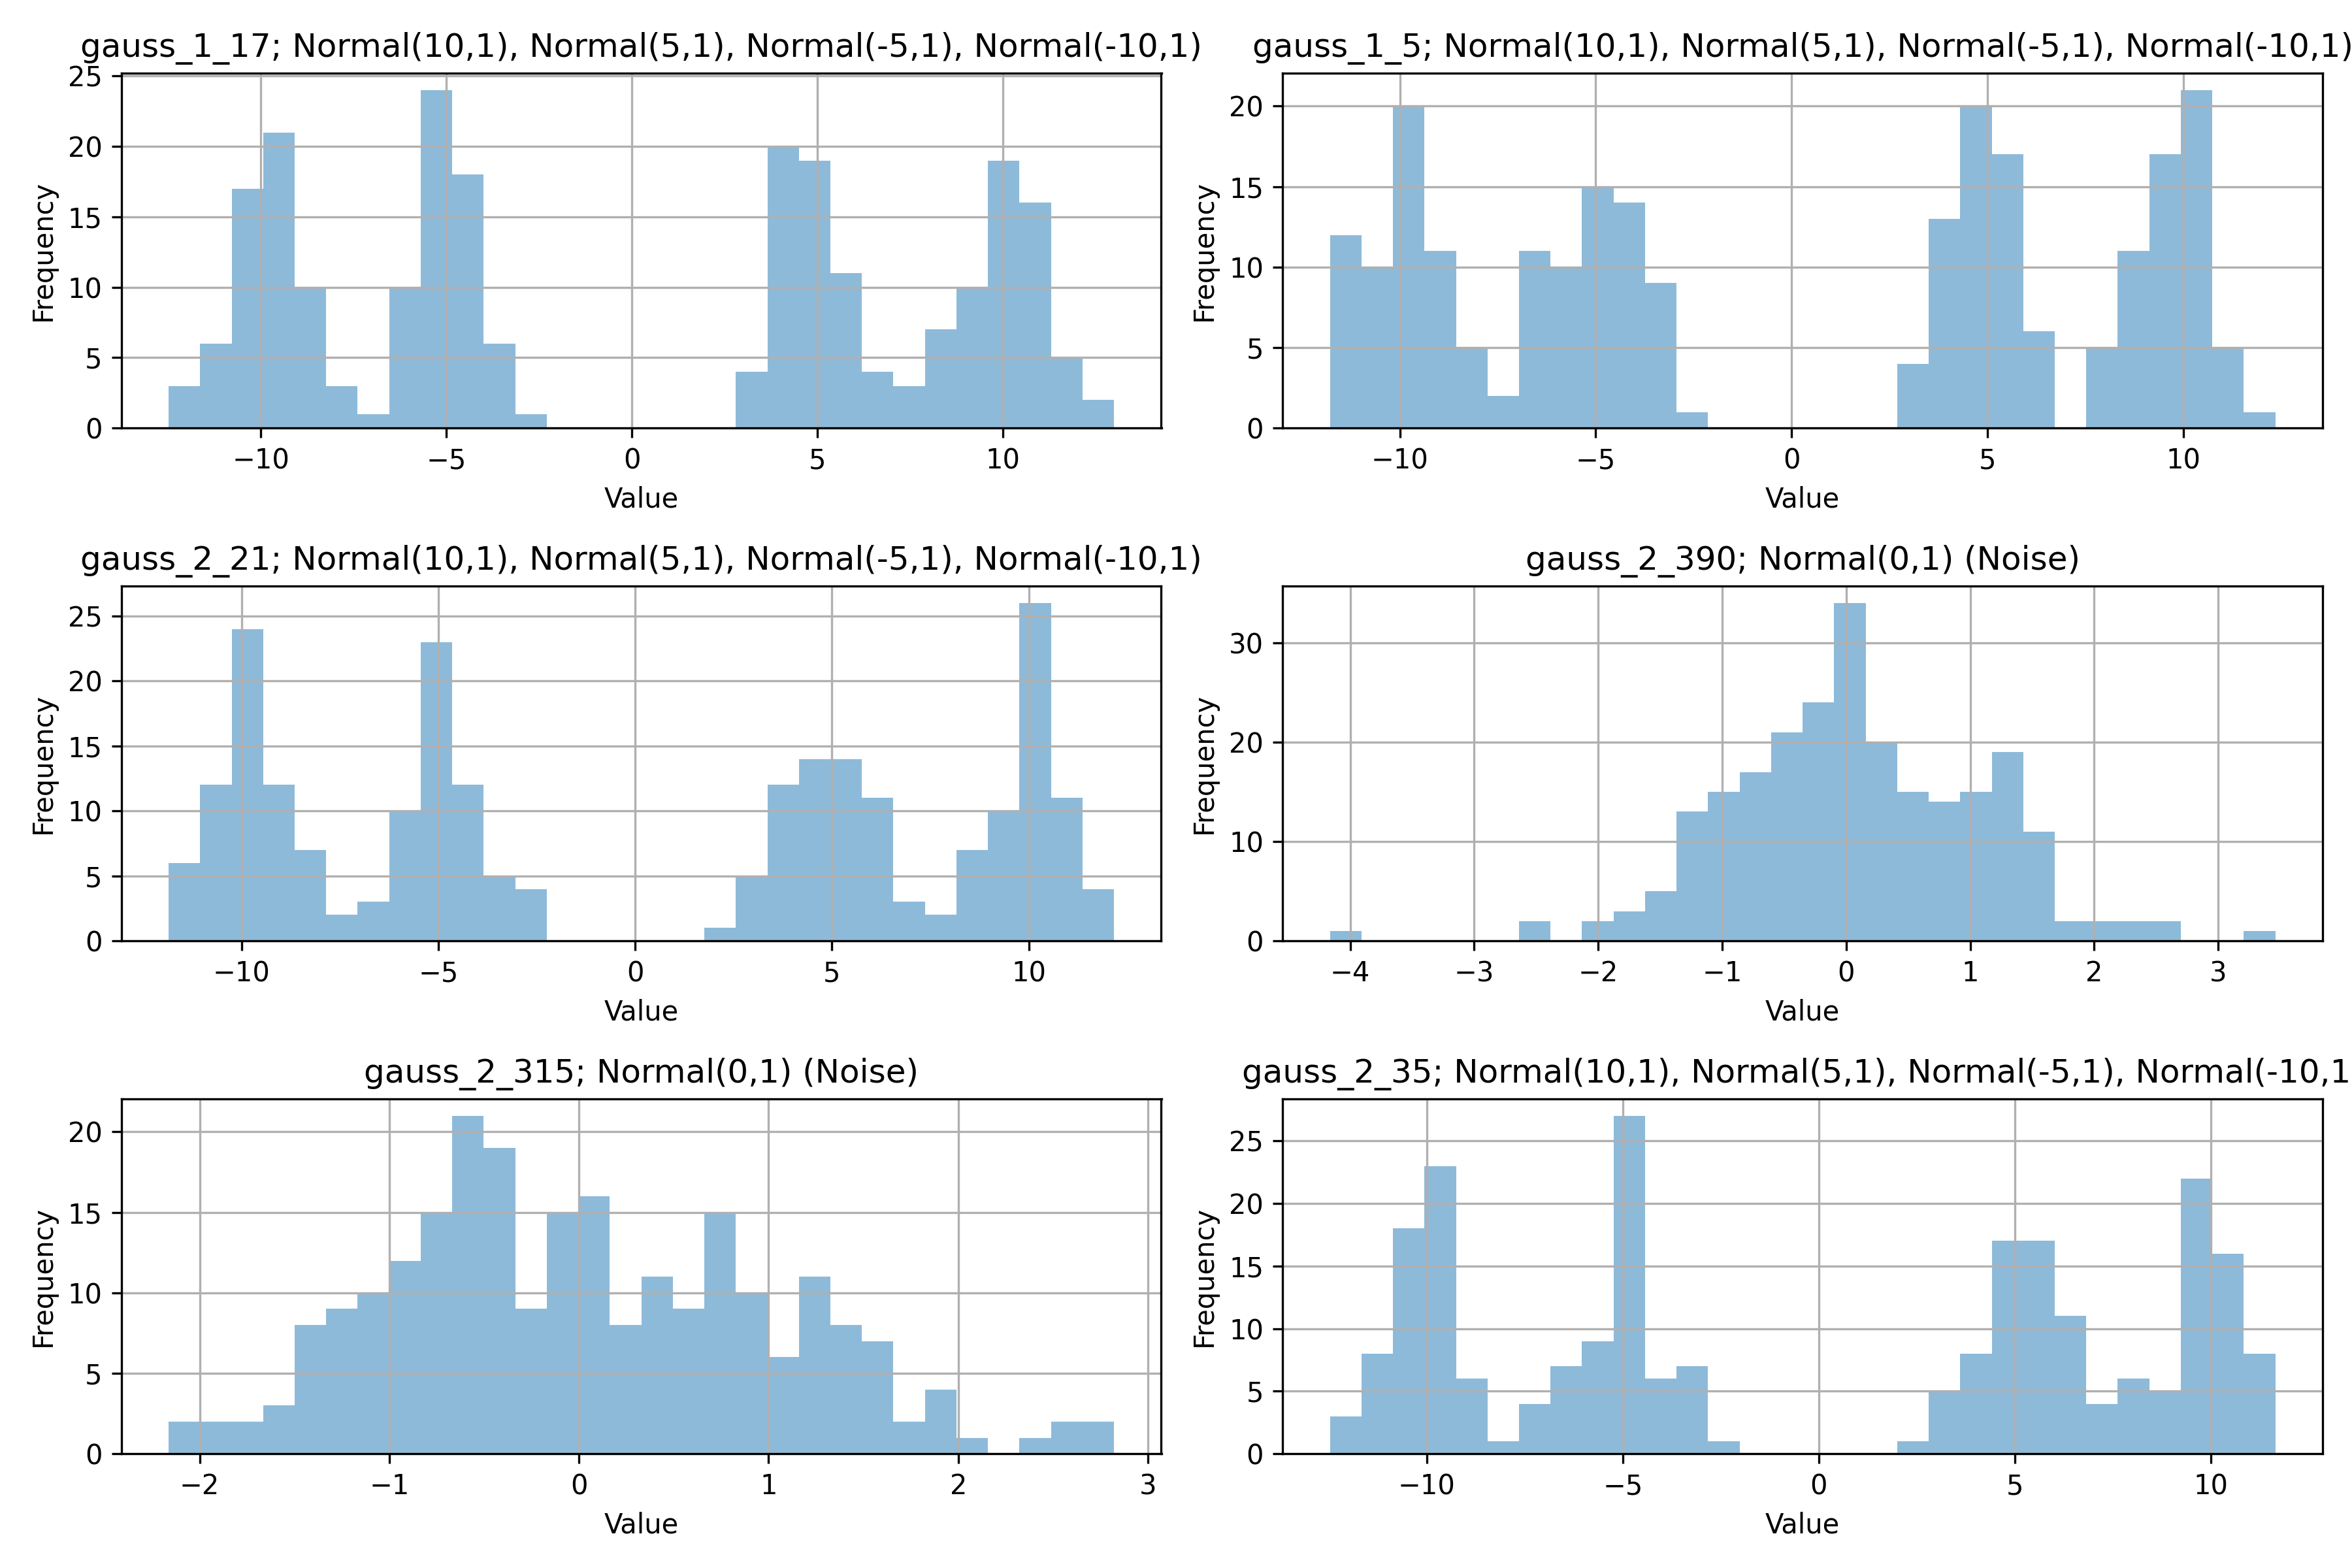
\includegraphics[width=0.9\linewidth]{../results/sim_valid_normal_distributions.png}
    \caption{Histograms of normal distributions that pass the normality test(correspond to table \ref{tab:normal_metrics})}
    \label{fig:normal_histograms}
\end{figure}

Figure~\ref{fig:normal_histograms} displays histograms of variables simulated from normal distributions.
Variables with titles including "(Noise)" correspond to noise components sampled from $\mathcal{N}(0,1)$,
while those without such a label represent relevant features derived from mixtures of $\mathcal{N}(10,1)$, 
$\mathcal{N}(5,1)$, $\mathcal{N}(-5,1)$, and $\mathcal{N}(-10,1)$. 
These relevant variables show clear multimodal patterns, indicating the presence of structured information.
In contrast, the noise variables exhibit unimodal, symmetric distributions centered around zero, 
lacking informative structure. The absence of "(Noise)" in the title marks the variables that
passed the normality test and were deemed statistically significant for downstream modeling.

\begin{figure}[!h]
    \centering
    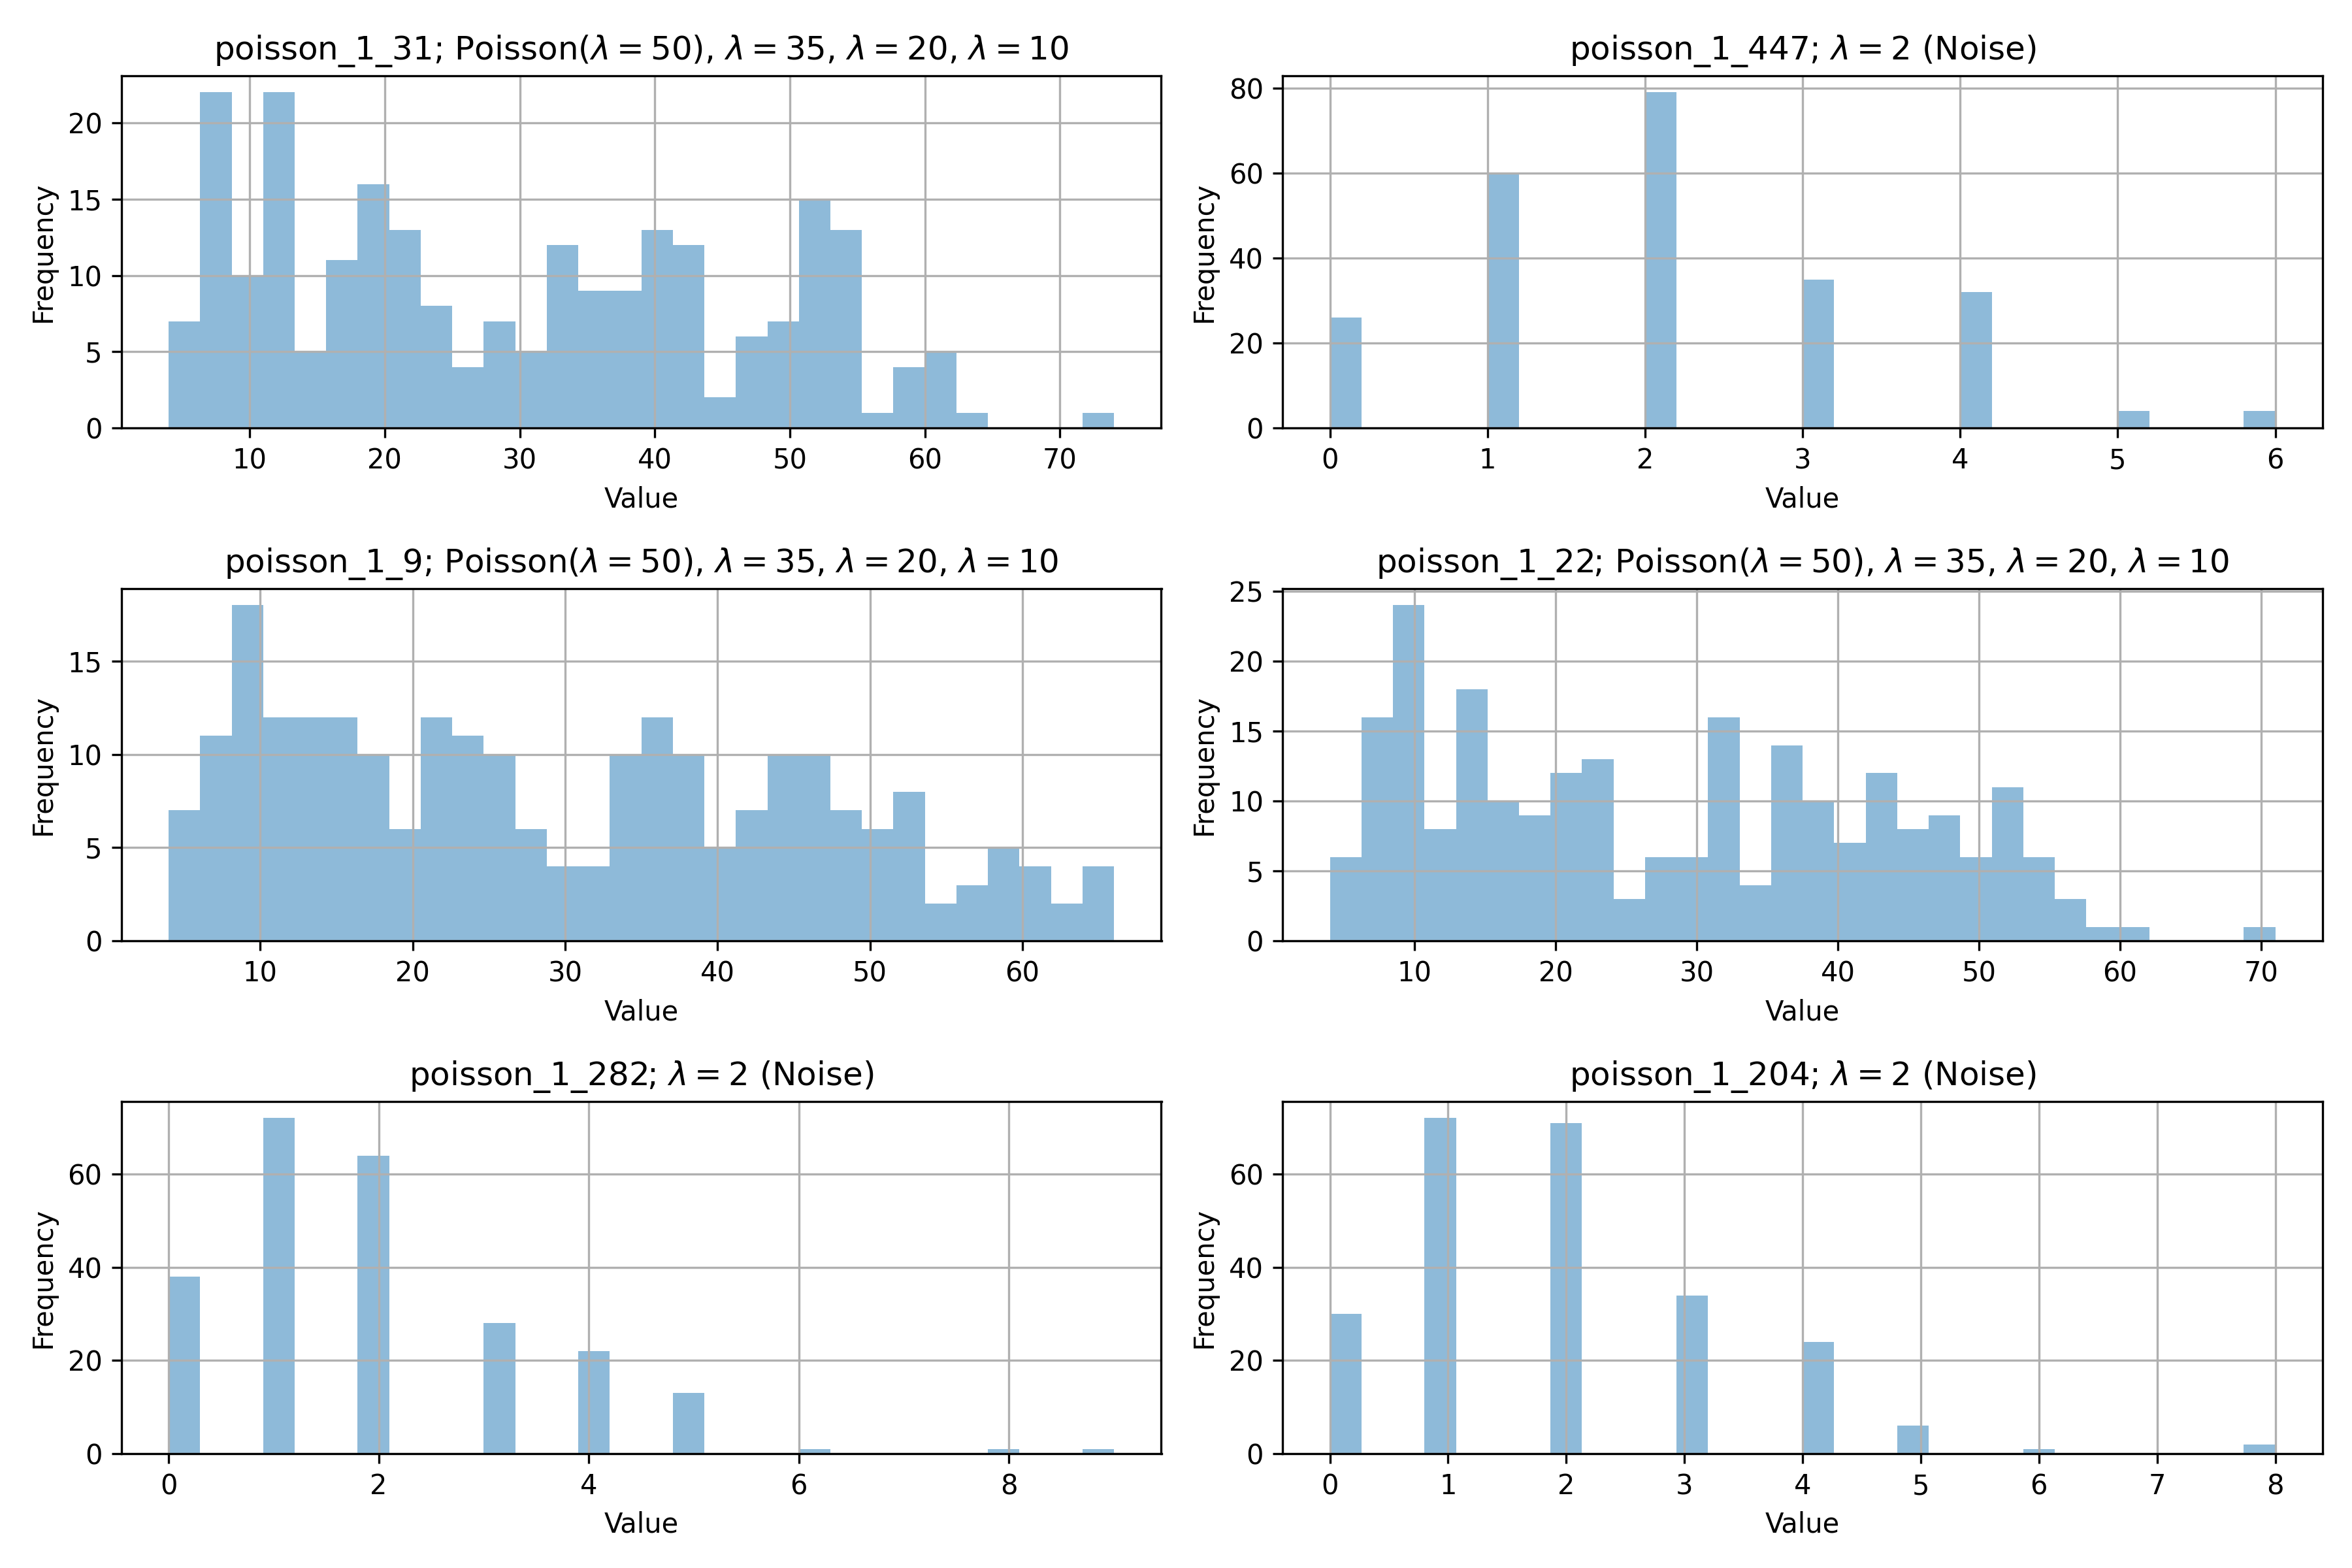
\includegraphics[width=0.9\linewidth]{../results/sim_valid_poisson_distribution.png}
    \caption{Histograms of normal distributions that pass the poission test (corresponding to table \ref{tab:poisson_metrics})}
    \label{fig:poisson_histograms}
\end{figure}

Figure~\ref{fig:poisson_histograms} shows histograms of variables generated from Poisson distributions with different
rate parameters $\lambda$. Variables labeled with multiple $\lambda$ values (e.g., $\lambda = 50, 35, 20, 10$) 
represent informative features composed of mixed Poisson signals. These histograms exhibit broader, multi-modal 
or skewed distributions, suggesting meaningful variability across groups, which is useful for clustering tasks. 
In contrast, variables marked as "(Noise)"—such as those with $\lambda = 2$ only—display narrow, 
concentrated distributions around small integer values. These noise variables do not carry discriminative 
structure and are thus considered irrelevant for clustering.

\subsection{Necessity of testing in EDA for iClusterVB algorithm}

The testing operations described above (numerical information are stored in tables \ref{tab:normal_metrics}, \ref{tab:poisson_metrics}, \ref{tab:bernoulli_metrics} in appendix) demonstrate the effectiveness of statistical tests 
in identifying suitable variables for downstream analysis. By applying normality, Poisson, and multinomial tests,
we were able to filter out irrelevant noise features and retain only the informative variables that 
exhibit meaningful patterns or variability. These selected variables are well-suited for integrative clustering 
and feature selection tasks, making them ideal candidates for input into the \texttt{iClusterVB} algorithm. 
This ensures that the algorithm operates on high-quality data, enhancing its ability to uncover biologically
meaningful clusters and informative features.



% Exploratory Data Analysis (EDA) is an important first step when working with data, especially high-dimensional data such as biological or medical datasets. EDA helps us to understand the structure of the data and to prepare it for further analysis like clustering and feature selection.

% We used EDA to look at how the data is distributed, find missing values or outliers, and see how variables relate to each other. This is useful before we apply clustering algorithms or choose important features. The methods we used here is basic  histograms or kde for each cluster. 

% \textcolor{red}{Starting here, using resampling method to check the distribution of the simulated data}


% \clearpage
% \subsection{Breast Cancer (TCGA) dataset}
% The breast cancer dataset used in this analysis was obtained from The Cancer Genome Atlas (TCGA) portal, specifically the TCGA-BRCA project, which provides comprehensive genomic data for breast cancer research. The dataset can be accessed at \url{https://portal.gdc.cancer.gov/projects/TCGA-BRCA}. This dataset includes multi-omic data, including gene expression, DNA methylation, and miRNA expression for 348 individuals diagnosed with breast cancer. The analysis was conducted using the \texttt{iClusterVB} framework, which leverages variational Bayesian inference for integrative clustering. The R code used in the analysis involved loading the necessary multi-omic data sets, specifying the clustering parameters (such as the number of clusters and feature selection method), and fitting the model using the \texttt{iClusterBayes} function. The model's posterior distributions were approximated using variational inference, and the results were visualized through heatmaps and posterior inclusion probability plots to identify informative features and cluster memberships. The \texttt{iClusterVB} framework effectively captured the heterogeneity within the dataset, revealing biologically meaningful subtypes of breast cancer based on molecular data.

